\begin{figure}[t]
\uwsinglespace
\begin{center}
\begin{minipage}{0.4\textwidth}
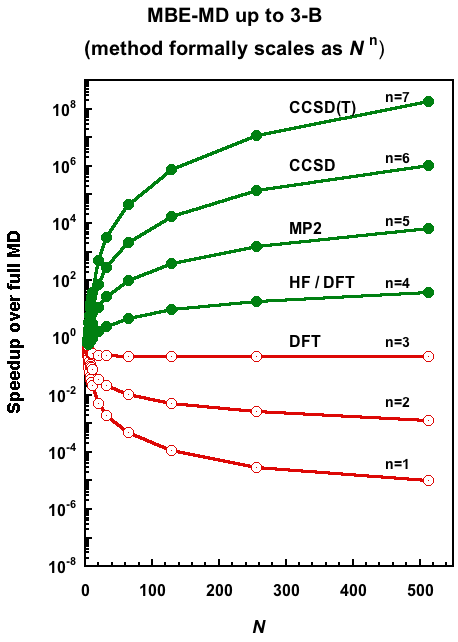
\includegraphics[width=\textwidth]{Figures/Chapter_4/ch4_figure_1_left.png}
\end{minipage}
\begin{minipage}{0.4\textwidth}
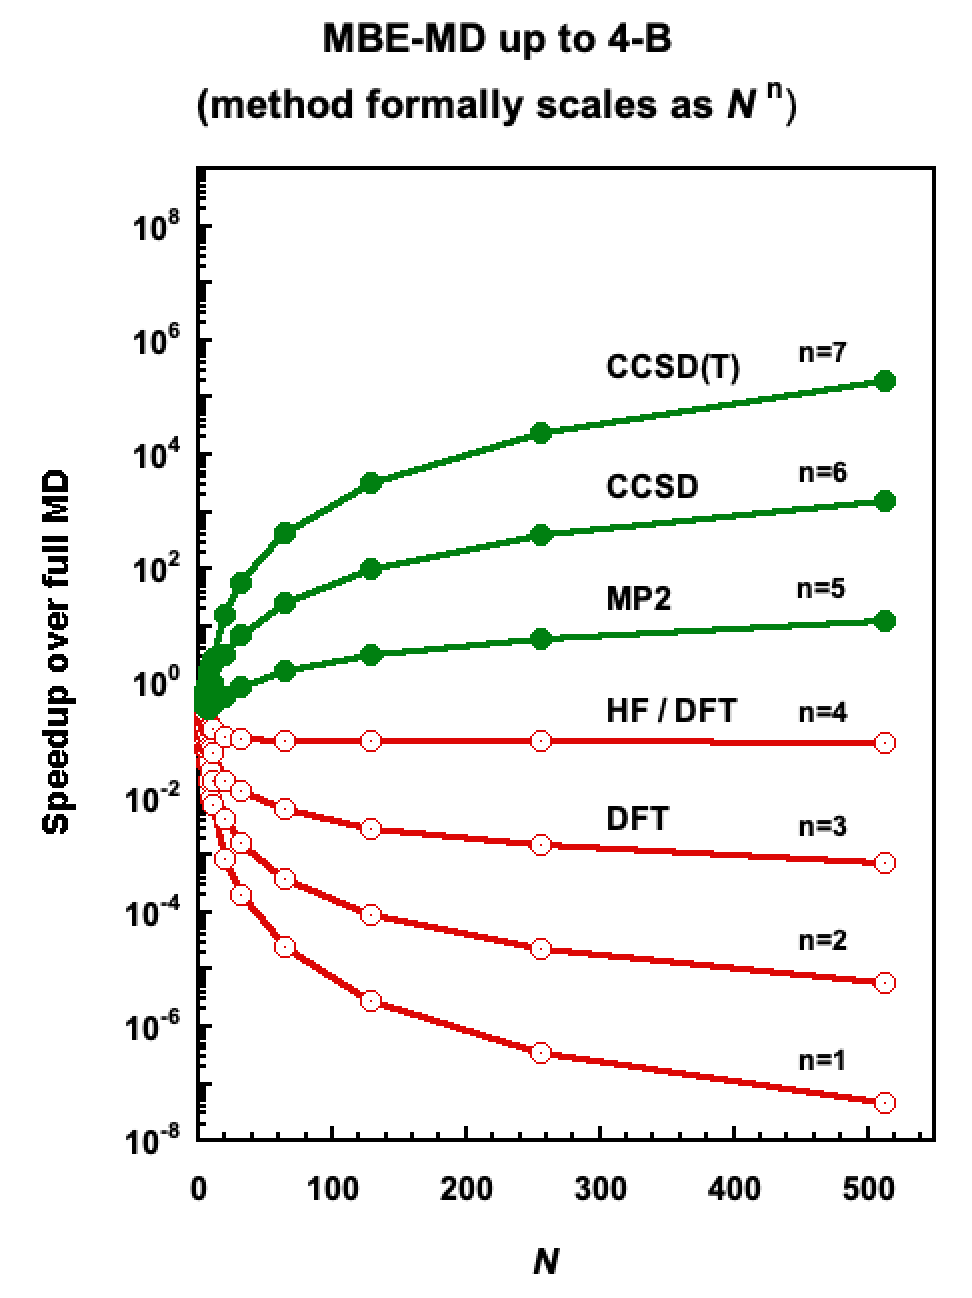
\includegraphics[width=\textwidth]{Figures/Chapter_4/ch4_figure_1_right.png}
\end{minipage}
\end{center}
\begin{spacing}{1.0}
\caption[Asymptotic speed-up of the MBE compared to a full calculation for varying numbers of fragments and various polynomial scaling of the relevant electronic structure method compared to a calculation on the full system. Each method is represented with a polynomial scaling as $N^n$, where $N$ is the number of fragments and $n$ the polynomial scaling exponent of the method in question.]{Asymptotic speed-up of the MBE compared to a full calculation for varying numbers of fragments and various polynomial scaling of the relevant electronic structure method compared to a calculation on the full system. Each method is represented with a polynomial scaling as $N^n$, where $N$ is the number of fragments and $n$ the polynomial scaling exponent of the method in question. Figure 1a assumes calculations are carried out to the 3-body term and Figure 1b to the 4-body term. Green/red lines indicate larger/smaller speedups with respect to the full calculation.}\label{fig:MBE_MD_F1_intro}
\end{spacing}
\end{figure}